\documentclass[UKenglish,aspectratio=169]{beamer}
\usepackage[utf8]{inputenc}
\usepackage{babel, textcomp}
\usepackage{arevtext}
\usepackage{microtype}

\usepackage{tikz}

\usepackage{amsmath, amssymb}
% \usepackage{caption}

\usepackage{hyperref}
\usepackage{xcolor}
% \hypersetup{ % this is just my personal choice, feel free to change things
%     colorlinks,
%     linkcolor={red!50!black},
%     citecolor={blue!50!black},
%     urlcolor={blue!80!black},
% }

\usetheme[
    uiostandard,
    font=none,
    % sectionsep=uiogreen2,
]{UiO}
\usefonttheme{professionalfonts}
\usefonttheme[onlymath]{serif}
\urlstyle{sf}

\title{FYS4480 Oral Exam}
\subtitle{Quantum mechanics for many-particle systems}
\author{August Femtehjell}
\uioemail{august.femtehjell@fys.uio.no}

\begin{document}
\uiofrontpage[
    % info={A minimal user guide},
    % image={uio-beamer-segl-pos},
    date={16th December, 2024},
]

\section{Introduction}
\begin{frame}{Notation}
    Here, we follow the notation of having states $ijk\ldots$ refer to occupied states, and $abc\ldots$ refer to unoccupied states, typically below and above the Fermi level, respectively.
    From a reference state $\lvert \Phi_0 \rangle$ with $N$ particles, we write a 1-particle-1-hole (1p1h) excitation as
    \begin{equation}
        \lvert \Phi_{i}^{a} \rangle
        = a_{a}^\dagger a_{i} \lvert \Phi_0 \rangle,
    \end{equation}
    and similarly for 2p2h, 3p3h, etc.
\end{frame}

\begin{frame}{Motivation}
    We are, in essence, interested in finding the ground state energy of a many-body system, that is, solving the eigenvalue problem
    \begin{equation}
        \hat{H} \lvert \Psi_0 \rangle = E_0 \lvert \Psi_0 \rangle,
    \end{equation}
    where $\hat{H}$ is the Hamiltonian operator and $\lvert \Psi_0 \rangle$ is the ground state wave function, such that the ground state energy $E_0$ is minimized.

    \bigskip

    The complexity arises from the fact that the exact solution cannot typically be found for systems with more than a few particles, and we must resort to approximations.
\end{frame}

\section{Full configuration interaction theory}

\begin{frame}{Full configuration interaction theory}
    In full configuration interaction (FCI) theory, we seek to write the wave function as a linear combination of all possible Slater determinants, that is, all possible configurations of the system, truncated at some level.

    \bigskip

    That is, we with to write the wave function as
    \begin{equation}
        \lvert \Psi_0 \rangle = C_0 \lvert \Phi_0 \rangle + \sum_{ia} C_i^a \lvert \Phi_i^a \rangle + \sum_{ijab} C_{ij}^{ab} \lvert \Phi_{ij}^{ab} \rangle + \ldots,
    \end{equation}
    where the coefficients $C$ are determined by solving the eigenvalue problem.
\end{frame}

\begin{frame}{Slater determinants for pairing model}
    \begin{figure}[htbp]
        \centering
        
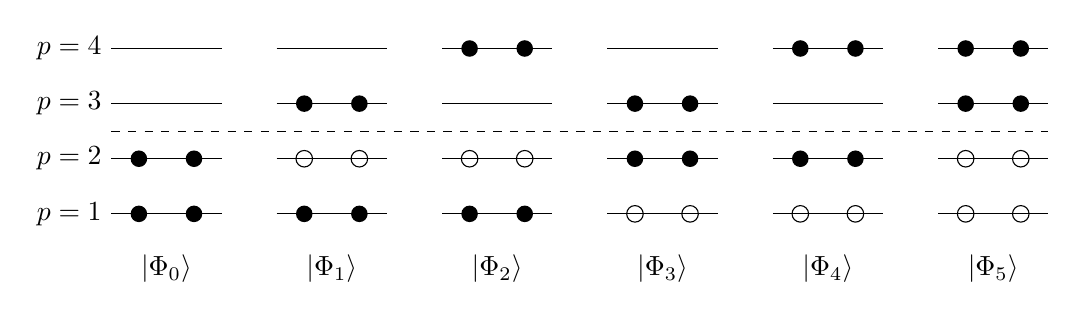
\begin{tikzpicture}[scale=0.7]
    % Draw lines
    \foreach \x in {0,3,6,9,12,15} {
        \foreach \y in {1,2,3,4} {
            \draw (\x, \y) -- (\x+2, \y);
        }
    }
    % Draw additional dashed lines
    \draw[dashed] (0, 2.5) -- (17, 2.5);

    % Labels on the left
    \foreach \y/\label in {1/$p=1$, 2/$p=2$, 3/$p=3$, 4/$p=4$} {
        \node[left] at (0, \y) {\label};
    }

    % Groundstate
    \foreach \x/\y in {0.5/1, 0.5/2, 1.5/1, 1.5/2} {
        \fill (\x, \y) circle (0.15);
    }
    \node at (1, 0) {$|\Phi_0\rangle$};

    % Phi_1
    \foreach \x in {3.5, 4.5} {
        \foreach \y in {1, 3} {
            \fill (\x, \y) circle (0.15);
        }
        \draw (\x, 2) circle (0.15);
    }
    \node at (4, 0) {$|\Phi_1\rangle$};

    % Phi_2
    \foreach \x in {6.5, 7.5} {
        \foreach \y in {1, 4} {
            \fill (\x, \y) circle (0.15);
        }
        \draw (\x, 2) circle (0.15);
    }
    \node at (7, 0) {$|\Phi_2\rangle$};

    % Phi_3
    \foreach \x in {9.5, 10.5} {
        \foreach \y in {2, 3} {
            \fill (\x, \y) circle (0.15);
        }
        \foreach \y in {1} {
            \draw (\x, \y) circle (0.15);
        }
    }
    \node at (10, 0) {$|\Phi_3\rangle$};

    % Phi_4
    \foreach \x in {12.5, 13.5} {
        \foreach \y in {2, 4} {
            \fill (\x, \y) circle (0.15);
        }
        \foreach \y in {1} {
            \draw (\x, \y) circle (0.15);
        }
    }
    \node at (13, 0) {$|\Phi_4\rangle$};

    % Phi_5
    \foreach \x in {15.5, 16.5} {
        \foreach \y in {3, 4} {
            \fill (\x, \y) circle (0.15);
        }
        \foreach \y in {1, 2} {
            \draw (\x, \y) circle (0.15);
        }
    }
    \node at (16, 0) {$|\Phi_5\rangle$};

\end{tikzpicture}

        \caption{
            Schematic representation of the six possible Slater determinants for a system with four particles, under the constraint of no broken pairs, total spin $S = 0$, considering only the four lowest levels $p = 1, 2, 3, 4$.\label{fig:SDs}
        }
    \end{figure}
\end{frame}

\begin{frame}{Solving the problem}
    In solving the system, one first has to set up the Hamiltonian matrix, with elements
    \begin{equation}
        H_{i, j} = \langle \Phi_i \lvert \hat{H} \rvert \Phi_j \rangle,
    \end{equation}
    and then diagonalize the matrix to find the eigenvalues and eigenvectors.
    The ground state energy can then be found as the lowest eigenvalue, with the corresponding eigenvector giving the coefficients $C$.

    \bigskip

    FCI is exact, but computationally expensive, as the number of configurations grows factorially with the number of energy levels included.
    Approximative methods are therefore required.
\end{frame}

% \begin{frame}
%     The method consists of the following steps:
%     \begin{enumerate}
%         \item Choose a basis set $\lvert \psi_i \rangle$.
%         \item Construct the Hamiltonian matrix.
%         \item Diagonalize the Hamiltonian matrix.
%         \item Calculate the expectation value of the energy.
%     \end{enumerate}

%     \bigskip

%     The method is exact as it includes all possible configurations of the system, but it is computationally expensive.

%     \begin{equation*}
%         -\frac{1}{2} \sum_{\substack{ab \\ ijkl}} \frac{
%             \langle li \vert V \vert lk \rangle
%             \langle kj \vert V \vert ab \rangle
%             \langle ab \vert V \vert ij \rangle
%         }{
%             (
%                 \varepsilon_i + \varepsilon_j - \varepsilon_a - \varepsilon_b
%             )(
%                 \varepsilon_k + \varepsilon_j - \varepsilon_a - \varepsilon_b
%             )
%         }
%     \end{equation*}
% \end{frame}

\section{Hatree-Fock theory}

\begin{frame}{Hatree-Fock theory}
    In Hatree-Fock theory, we seek to write the wave function as a single Slater determinant, that is, a single configuration of the system.

    \bigskip

    The wave function is then written as
    \begin{equation}
        \lvert \Psi_0 \rangle = \lvert \Phi_0 \rangle,
    \end{equation}
    where $\lvert \Phi_0 \rangle$ is the Slater determinant that minimizes the energy.

    \bigskip

    The Hatree-Fock method is a variational method, and the energy is minimized by varying the coefficients in the Slater determinant.
\end{frame}

\section{Many-body pertubation theory}
\subsection{Brillouin-Wigner pertubation theory}
\subsection{Rayleigh-Schrödinger pertubation theory}

\section{Coupled-Clusted theory}

\end{document}
